\documentclass[12pt, letterpaper]{article}

\usepackage{parskip}
\usepackage{tikz}
\usetikzlibrary{shapes.geometric}


\begin{document}
\section*{Problem 1}
Two squares of side length 1 have a common centre $c$. Show that the area of their intersection is at least $\frac{3}{4}$\\

\begin{center}
\begin{tikzpicture}
\node[rectangle, rotate = -45,  draw,
	minimum width = 5cm,
	minimum height = 5cm] (d) at (0,0) {};
\node[rectangle, draw,
	minimum width = 5cm,
	minimum height = 5cm] (s) at (0,0) {};
\node[circle, draw, fill = black, inner sep=0pt, minimum size = 1pt] (c) at (s.center) {};
\node[yshift = -0.25cm, xshift = 0.25cm] at (c) {$c$};
\end{tikzpicture}
\end{center}

\newpage

\section*{Solution}
We gain insight by observing the two squares are identical, except one is rotated 45 degrees. This means we can inscribe a circle inside one square, and the same circle will perfectly inscribe the second square, like so: \\ 

\begin{center}
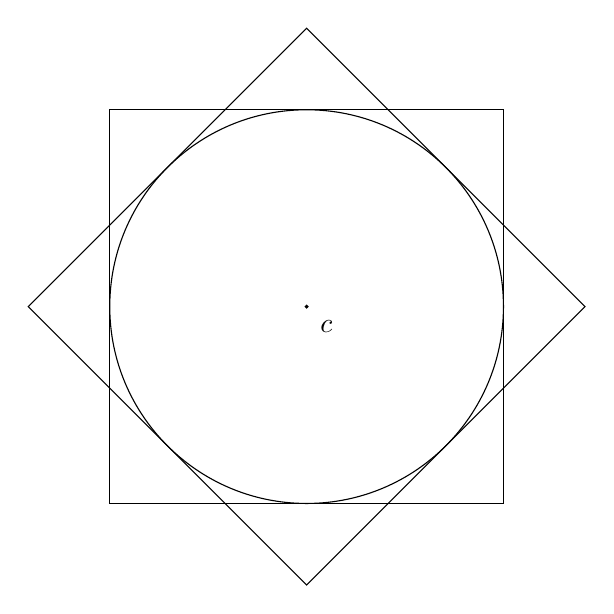
\begin{tikzpicture}
\node[rectangle, rotate = -45,  draw,
	minimum width = 5cm,
	minimum height = 5cm] (d) at (0,0) {};
\node[rectangle, draw,
	minimum width = 5cm,
	minimum height = 5cm] (s) at (0,0) {};
\node[circle, draw, fill = black, inner sep=0pt, minimum size = 1pt] (c) at (s.center) {};
\node[yshift = -0.25cm, xshift = 0.25cm] at (c) {$c$};
\node[circle, draw, minimum size = 5cm] (circle) at (0,0) {};
\end{tikzpicture}
\end{center}

We conclude that the area of the intersection must be at least the area of the circle.

We know the radius of the circle is $\frac{1}{2}$ and so the area is $\pi \cdot (\frac{1}{2})^2 = \frac{\pi}{4}$

We then have $\frac{\pi}{4} > \frac{3}{4}$, completing the proof.


\end{document}
